\section{Blockchain structure}

In this part, we'll try to understand in more detail the blockchain's components and how they work together.

Bitcoin is a specific implementation of the blockchain but it's the starting point of our analysis. \newline

As we mentioned before, the blockchain is based on decentralized implementation. Actually, it's based on a peer-to-peer network.

\begin{figure}[ht]
\centering
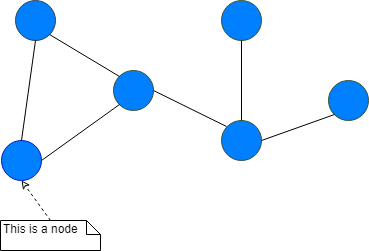
\includegraphics[width=4cm]{Figures/network}
\caption{Peer-to-peer network}
\end{figure}
\medskip

Each node has three responsibilities :

\begin{itemize}
  \item Keeping a copy of confirmed transactions, which is the blockchain itself.
  \item Validating a transaction if it's following the rules.
  \item Sharing information with their neighbors such as unconfirmed but valid transactions and mined blocks.
\end{itemize}

\clearpage

\begin{aside}

\paragraph{C ++ Code}

We've written a C++ code to simulate blockchains focusing on the mining process. The code is written in C++ using the library MPI to parallelize the process. Moreover, the executions were made on the Geneva University cluster to truly parallelize the code.

A full part is dedicated to the results we found in these simulations. \newline

Thus, we can simulate several miners trying to mine blocks and keep the blockchain synchronized. The goal is to deeply understand the network structure and to observe the evolution of the blockchain in the time. \newline

All along with the presentation of the blockchain's principles, we'll show the implementation in our code.

\end{aside}
\medskip

  \subsection{Transaction}

The main feature of the blockchain is to record transactions.

A transaction is composed of a list of inputs and a list of outputs (see Figure~\ref{transaction}). Outputs can include the payer itself. \newline

While doing a transaction, one wants to be sure that the payer is the true owner of the money. Then, to check this,  we use digital signatures :

\begin{itemize}
  \item The inputs of the transaction are encrypted with the public key of the payer.
  \item To prove he owns the coins, the payer "unlock" them by decrypting the signature with his private key.
  \item Then, he "locks" the outputs with the public key of the payees.
\end{itemize}

Technically, this is done with scripts linked to each input and output (see \cite{broken_crypto_primitives} for more details).


\begin{figure}[ht]
\centering
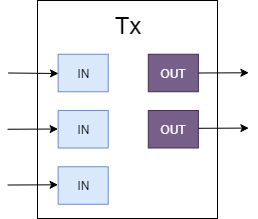
\includegraphics[width=4cm]{Figures/Transaction}
\hspace{1cm}
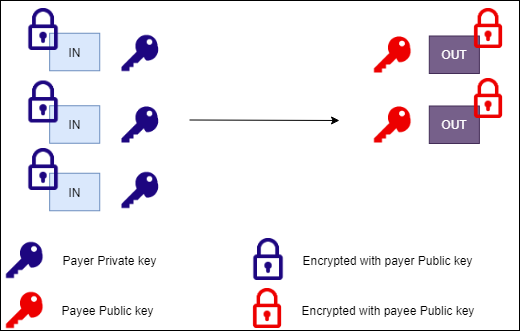
\includegraphics[width=8cm]{Figures/Transaction2}
\caption{A transaction diagram and digital signatures}
\label{transaction}
\end{figure}
\medskip

\begin{aside}

\paragraph{C++ code}

As we mentioned, the code focus on the mining process so we've simplified transaction management. \newline

In our simulation, a transaction is just a string, for example: (each line is a transaction) \newline

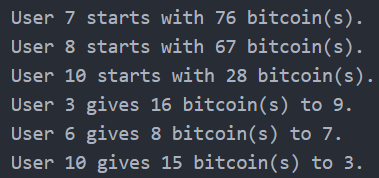
\includegraphics[width=6cm]{Figures/transactionsExample}
\medskip

So we don't have to manage signatures, inputs and outputs and it won't affect the mining process.

\clearpage

To generate those transactions, we've created a specific generator which creates a given number of transactions with limitations in the amount of money exchanged for a given number of users. \newline

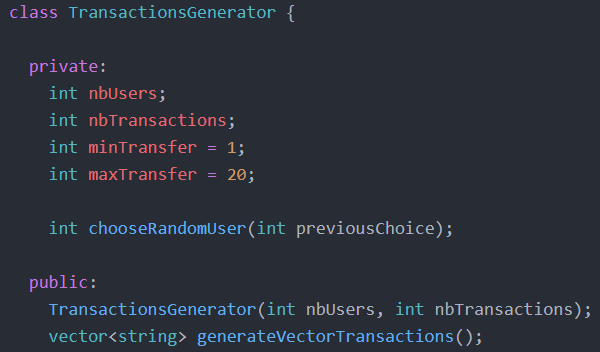
\includegraphics[width=10cm]{Figures/ClassTransactionsGenerator}
\medskip

\end{aside}
\medskip


  \subsection{Block}

Now that we have a transaction, we can transmit it to a node of the network. There, it needs to pass verification and if it's correct, it will be broadcast to other nodes. \newline

Once the transaction is accepted by a node, it will stay in a special area called the Mempool (Memory pool), this is where all unconfirmed transactions wait to be added in a block. A node can prioritize the transactions in its Mempool, especially if he's running out of memory, he can choose the order of arrival or, more probably, the highest transaction fee.

When a node receives the information that a new block has been added to the blockchain, he removes all newly confirmed transactions from his Mempool.  \newline

To form a new block candidate, a miner gathers transactions from the Mempool. Then, he will try to mine this block to add it to the blockchain. The miner will also add a block header which gives more information about the block (see \ref{blockHeader}). \newline

\begin{figure}[ht]
\centering
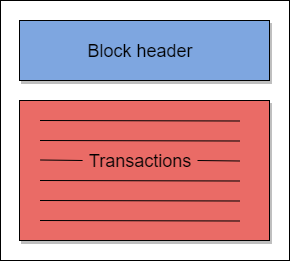
\includegraphics[width=4cm]{Figures/block}
\caption{A transaction diagram and digital signatures}
\end{figure}
\medskip

\begin{aside}

\paragraph{C++ code}

A block is an object with the following fields: \newline

\begin{itemize}
  \item A vector of string representing the transactions.
  \item A block header (see explanations below).
  \item An ID to get its position in the blockchain.
  \item We also add a reference to the previous block, this is used to build the blockchain.
\end{itemize}
\medskip

\clearpage
\medskip
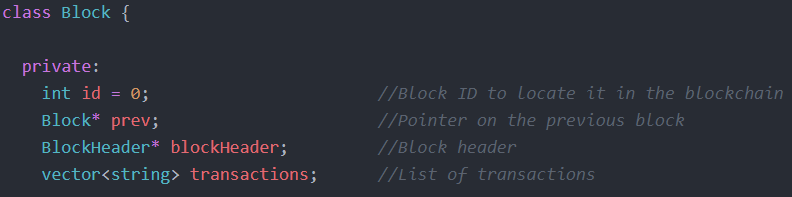
\includegraphics[width=10cm]{Figures/ClassBlock}
\medskip

A block can also build the Merkle tree with its transactions and be added in a blockchain.

\end{aside}
\medskip

  \subsection{Block header} \label{blockHeader}

A block header is a summary of the block, it's like its metadata. A block header contains six fields: \newline

\begin{tabular}{lll}
   version & The block's version & 4 bytes\\
   hashPrevBlock & The previous block's hash & 32 bytes \\
   hashMerkleRoot & The Merkle root representing all transactions in the block (see \ref{merkleRoot}) & 32 bytes \\
   time & The Unix time at which the block header was hashed & 4 bytes \\
   target & This is a shortened version of the target (see \ref{target}) & 4 bytes \\
   nonce & A random number  & 4 bytes \\
\end{tabular}

We'll see later that block headers are used for mining (see \ref{mining}).

\begin{aside}

\paragraph{C++ code}

As we've just seen, a block header contains all the fields mentioned: version, previous block hash, Merkle root, time, target and the nonce. \newline

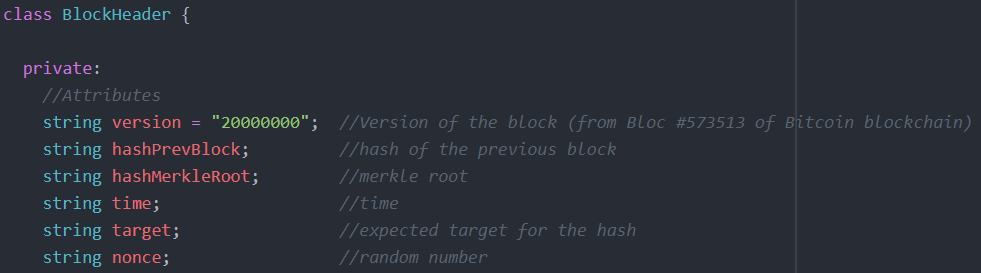
\includegraphics[width=14cm]{Figures/ClassBlockHeader}
\medskip

The version is always the same in our simulation because it won't affect mining. In the real world, the version helps to decode the block. A block header can set a nonce and compute its hash (by applying SHA256 twice).

\end{aside}
\medskip

  \subsection{Merkle root} \label{merkleRoot}

  As we've just seen, one of the block header fields is a Merkle root. Conceptually, it represents a fingerprint of the transactions' list and concretely it's just a hash.

  The blockchain uses Merkle trees for two reasons :

  \begin{itemize}
    \item To have a lightweight representation of the transactions because it results in only a hash.
    \item To be able to check if a transaction exists in a block without knowing all transactions in this block.
  \end{itemize}

  Merkle trees use a hash function, for blockchains, they use the same function than mining, which is

  SHA256(SHA256(.)).

  \begin{figure}[ht]
  \centering
  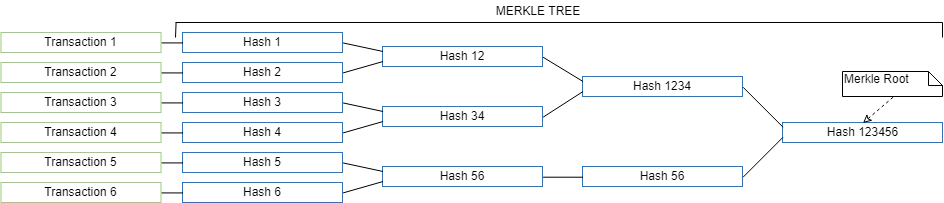
\includegraphics[width=\textwidth]{Figures/merkleTree}
  \caption{A Merkle tree}
  \end{figure}
  \medskip

  The main advantage of this technology is the speed and the ease to verify if a transaction belongs to a block. We don't need to know all transactions of the block and we don't even need to reveal any data from the transactions but only their hashes. \newline

  For example, if we want to check if the transaction 3 belongs to the block in our previous figure. We have to know its hash (Hash 3), Hash 4, Hash 12 and Hash 56. With those hashes, we can reconstruct the Merkle root. If it's the same, this means that the transaction 3 belongs to the block and that no transaction has been modified so the whole block is correct.


  \begin{aside}

  \paragraph{C++ code}

  We've created a class to build the Merkle tree from a vector of string and to return the Merkle root. \newline

  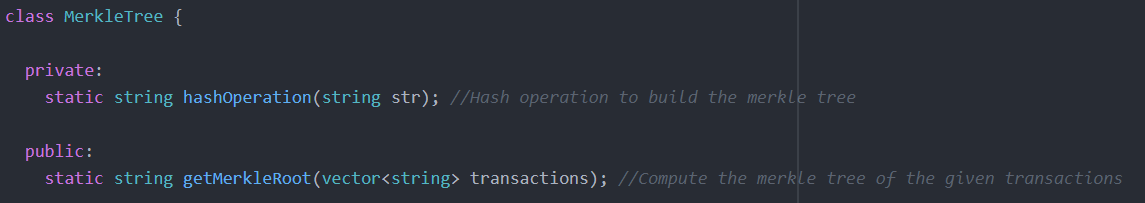
\includegraphics[width=14cm]{Figures/ClassMerkleTree}

  \end{aside}
  \medskip

  \subsection{The network}

  With all the concepts presented above, we can create a transaction, add it in a block, which will be mined thanks to its block header. Now, let's see how the nodes in the network secure the blockchain together. \newline

  The strength of the blockchain lies in its network because each node keeps a complete or partial copy of the blockchain. To keep the network updated, the nodes constantly share information between them. Typically, to broadcast a new transaction or a newly mined block :

  \begin{figure}[ht]
  \centering
  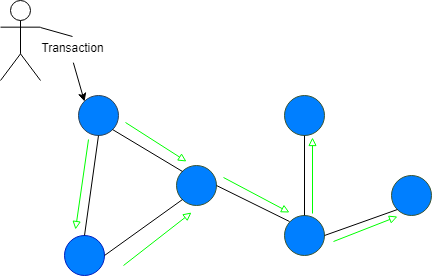
\includegraphics[width=5cm]{Figures/networkTransaction}
  \hspace{1cm}
  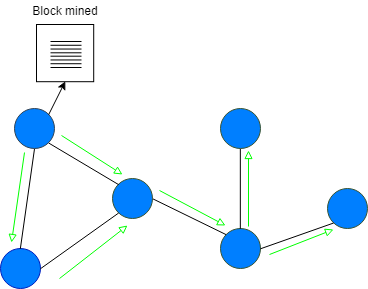
\includegraphics[width=5cm]{Figures/networkBlock}
  \caption{Communication inside the network}
  \end{figure}

  Then, each node updates its version of the blockchain. Now, one can wonder what happens if a node receives two different mined blocks at the same time?

  The node will fork the blockchain and have two versions of it and he will keep accepting blocks for both chains. As long as they have the same length, the node will choose to work on one of the chains but if one chain becomes longer, the node will keep it and forget the other one.

  \begin{figure}[ht]
  \centering
  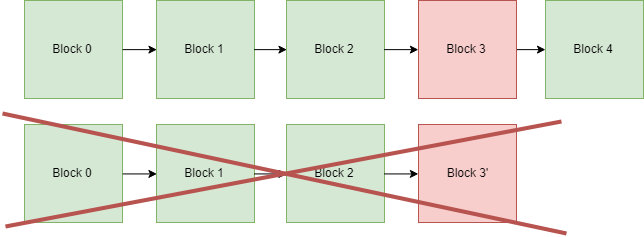
\includegraphics[width=5cm]{Figures/forkChains}
  \caption{Fork chains}
  \end{figure}

  The blockchain is always the longest chain created because it's the one that has requested more work of mining. This means that to have control over the blockchain, an attacker should have the majority of the computational power (at least 51\%). \newline

  \begin{aside}

  \paragraph{C++ code}

  As we said, the network is composed of miners so we implement mines as an object with the following fields: \newline

  \begin{itemize}
    \item An ID
    \item A vector of string to describe his mempool.
    \item A vector of blockchains to describe his versions of blockchains including forks.
  \end{itemize}
  \medskip

  \clearpage

  \medskip
  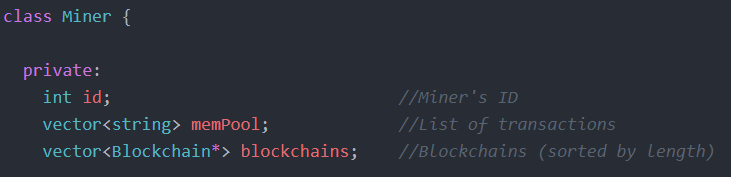
\includegraphics[width=10cm]{Figures/ClassMiner}
  \medskip

  A miner can fill a new block with transactions from his mempool, mine a block and add a block to one of his blockchains.

  Miners also have some functions to communicate through the network. For example, to serialize and deserialize blockchains (because only serializable objects can be sent in the network) or to handle a block the miner received. \newline

  Finally, blockchains are represented as linked lists with basic operations like adding a block or consult the last block. \newline

  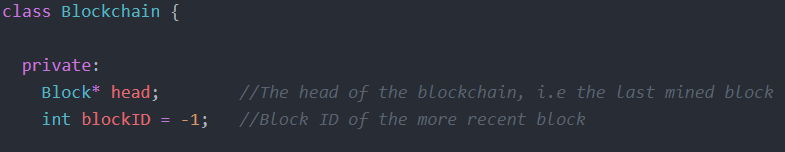
\includegraphics[width=10cm]{Figures/ClassBlockchain}

  \end{aside}
  \medskip

    \subsection{Bitcoin Block example}

  Bitcoin blockchain is public, we can follow the evolution on web sites like www.blockchain.com (\cite{blockchain_web_site}). We can see the fields we described and some other details, for example: \newline

  \begin{figure}[ht]
  \centering
  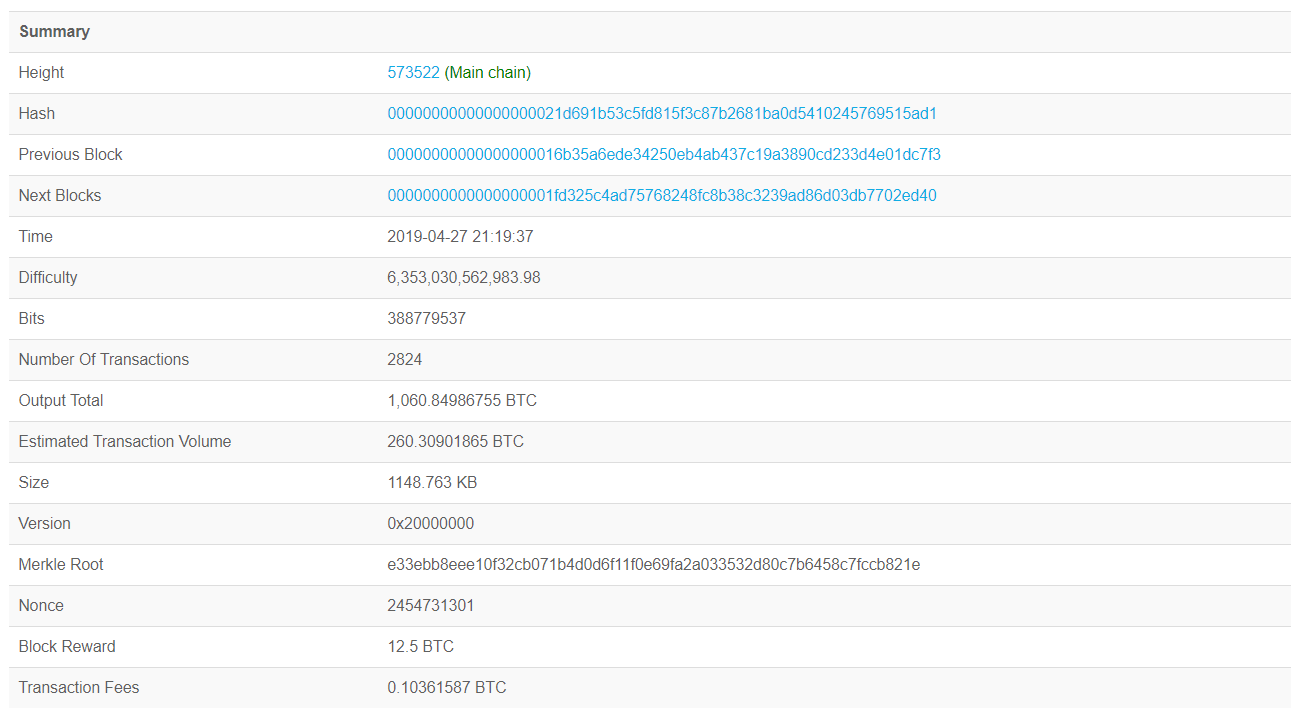
\includegraphics[width=15cm]{Figures/Block573522}
  \caption{Example of a Bitcoin block}
  \end{figure}

  \clearpage
